\section{WattDepot}

Software for energy collection, storage, and analysis tends to come in two flavors that support two ends of the scalability spectrum.  At one end are utility-scale SCADA systems and protocols which are intended to manage macro-grid data \cite{SmartEnergy2.0,OSHAN,OpenPDC}.  At the other end are ``personal scale'' systems such as those provided by energy meter or solar panel manufacturers which are intended to manage information about single households \cite{TED,EMS100}.  We designed WattDepot to support a middle ground that we refer to as ``enterprise-level'' energy management, in which data concerning energy production and consumption of hundreds to thousands of households can be usefully managed.  Figure \ref{fig:wattdepot} illustrates the architecture of the system, where WattDepot sensors send data from meters attached to energy devices to a server, which can then be queried by clients to provide visualizations and analyses.

\begin{figure}
\begin{center}
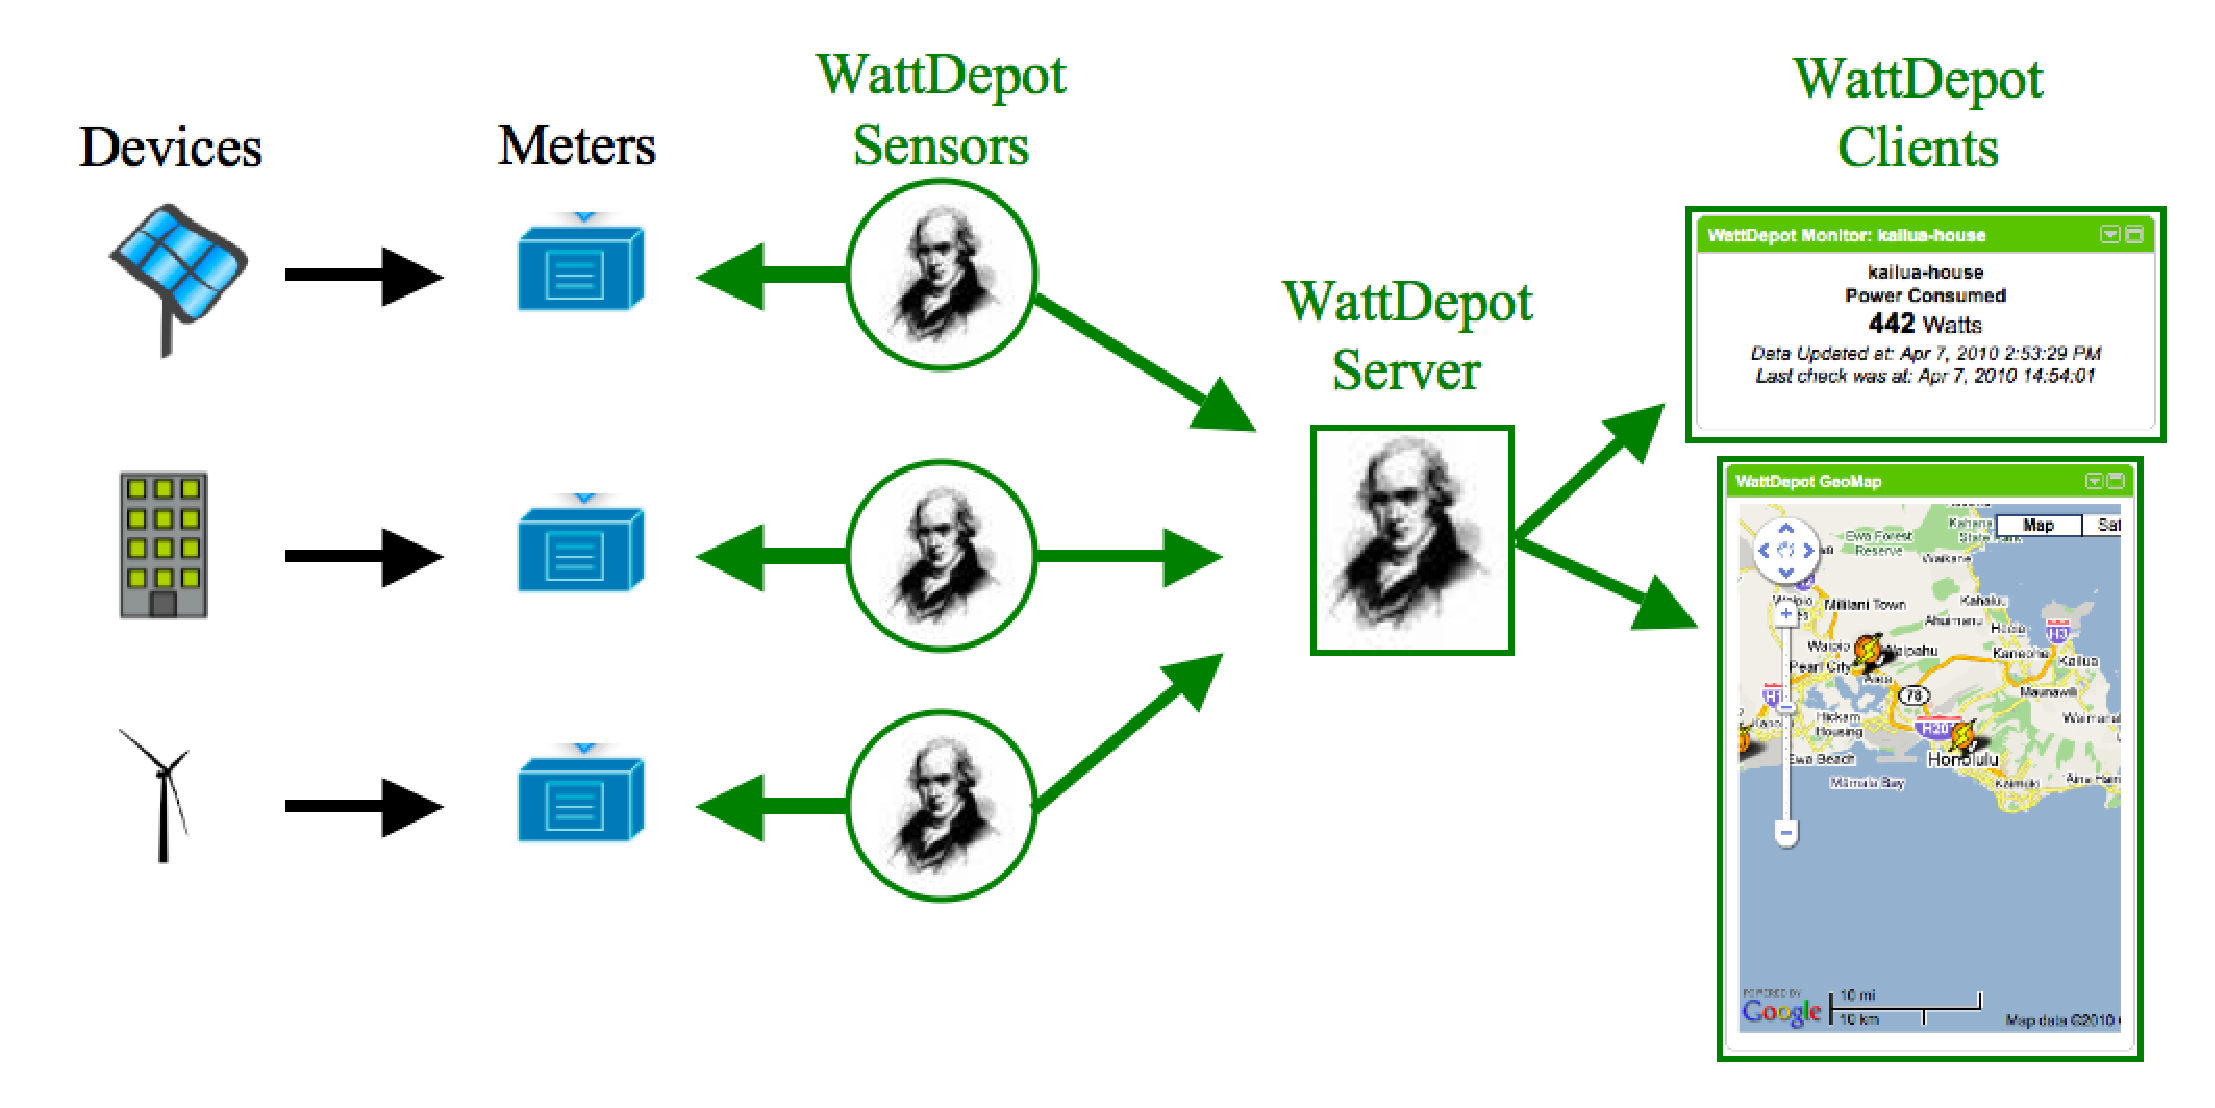
\epsfig{file=wattdepot-architecture, width=3in}
\end{center}
\caption{Architecture of WattDepot}
\label{fig:wattdepot}
\end{figure}

Our use of WattDepot has led to a novel set of capabilities to support this middle ground.

First, unlike personal-scale systems that are typically tied to a particular manufacturer's product, WattDepot is agnostic about the kinds of meters used to monitor energy production and consumption data, and whether the data is personal-scale or utility-scale. It provides a REST protocol for data transmission that can be used to implement clients for a wide variety of devices; the major constraint is that these devices need to have network access. WattDepot clients can be written in any language that supports the HTTP protocol. We provide a high-level client libraries for Java and JavaScript.

Second, WattDepot can represent aggregations of power sou\-rces. For example, a building might have multiple meters monitoring energy consumption, one per floor. WattDepot can represent the power consumed by individual floors, as well as an aggregate source representing the building as a whole. Aggregations can be nested, so that floors can be aggregated into buildings, buildings into neighborhoods, and neighborhoods into cities.

Third, WattDepot automatically performs data interpolation when necessary. For example, a meter might provide a snapshot of energy usage once per hour for a given device. Clients can request the power consumed by this device at any time instant, and WattDepot will automatically provide interpolation when the requested time does not match a time for which actual sensor data is available.

Fourth, WattDepot is architecturally decoupled from the underlying data storage technology. This supports experimentation with both traditional relational as well as NoSQL technologies, and facilitates scalability. Currently, WattDepot implements support for Derby, Postgres, and BerkeleyDB storage systems.

Fifth, WattDepot is designed to support both Platform-as-a-Service (PaaS) and local installation. We have successfully deployed WattDepot to the Heroku cloud-based hosting service.

Sixth, WattDepot implements support for ``ephemeral'' data. In some application scenarios, it is useful to send energy data to the WattDepot server quite frequently (i.e. every few seconds) so that clients can monitor current energy consumption with low latency. However, that rate of data sampling is not necessary for historical analyses, which may only require energy data sampling at the rate of every few minutes. WattDepot supports this situation through ephemeral data, which creates an in-memory window during which all recently received energy data is available for retrieval, but stored in the repository only at a much lower sampling rate.

Finally, WattDepot can be effectively used for simulation and what-if scenario development, as well as for management of live energy data.  This makes it appropriate as a kind of technological ``scaffolding'' for smart grid applications, where WattDepot can provide clients with simulated production and consumption data early in development, with the simulated data transitioning to live data as these sources go online later in development.
